\begin{explanationbox}
\textbf{先看标准图：$a=5,\ b=3,\ c=4,\ \theta=60^\circ$。}
\begin{center}
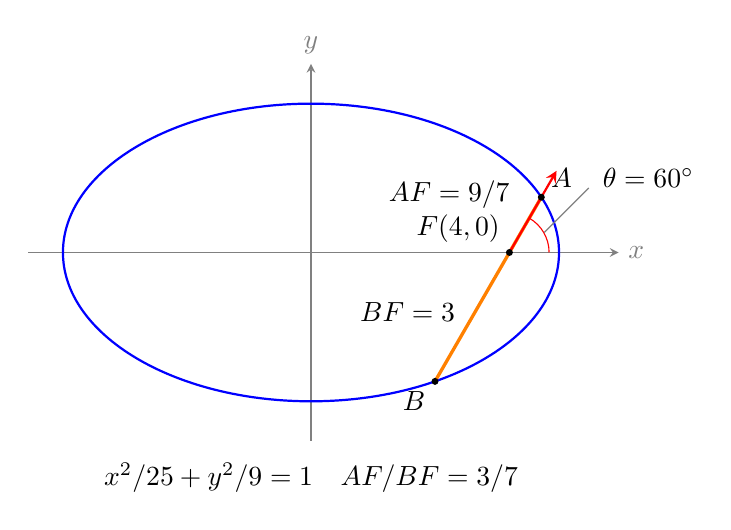
\begin{tikzpicture}[scale=.63,>=stealth]
\draw[->,gray] (-5.7,0)--(6.2,0) node[right] {$x$};
\draw[->,gray] (0,-3.8)--(0,3.8) node[above] {$y$};
\draw[blue,thick] (0,0) ellipse (5 and 3);
\coordinate (F) at (4,0); \coordinate (A) at ({65/14},{9*sqrt(3)/14});
\coordinate (B) at (2.5,{-3*sqrt(3)/2});
\draw[orange,very thick] (B)--(A);
\draw[->,red,thick] (F)--({4+1.9*.5},{1.9*sqrt(3)/2});
\draw[red] (4.8,0) arc (0:60:.8);
\draw[gray] (4.7,.4)--(5.6,1.3);\node at (6.8,1.5) {$\theta=60^\circ$};
\fill (F) circle (2pt) node[above left] {$F(4,0)$};
\fill (A) circle (2pt) node[above right] {$A$};
\fill (B) circle (2pt) node[below left] {$B$};
\node[left] at (3.1,-1.2) {$BF=3$};
\node[above left] at (4.2,.7) {$AF=9/7$};
\node[align=center] at (0,-4.55) {$x^2/25+y^2/9=1$\quad $AF/BF=3/7$};
\end{tikzpicture}

\end{center}
\textbf{一句话直觉：右焦点出发，朝右的半弦短，朝左的半弦长。}
右焦点 $F=(c,0)$ 已靠近椭圆右端点。
当 $\theta$ 为锐角时，$A$ 相对于 $F$ 向右走，$B$ 向左走，
因此 $AF<BF$；公式应呈现
$AF$ 分母\textbf{加} $c\cos\theta$、$BF$ 分母\textbf{减} $c\cos\theta$。
但当 $\theta$ 为钝角时，$A$ 恰好位于向左的方向，长短关系会反过来。
\par\smallskip\noindent
\textbf{为什么仅看 $\cos\theta$？}
对于距离 $F$ 为 $r$ 的点 $A$，横坐标的变化是 $r\cos\theta$；
沿反方向走 $s$ 到 $B$，横坐标的变化是 $-s\cos\theta$：
\[
 x_A=c+r\cos\theta,\qquad x_B=c-s\cos\theta.
\]
\textbf{只看横向投影}就能判断它们与右准线的距离；
椭圆第二定义说``到焦点距离／到对应准线距离 $=e$''，
从而产生只含 $r$ 或 $s$ 的一次方程。
\par\smallskip\noindent
\textbf{两端特例，是最可靠的正负号检查：}
\begin{enumerate}
 \item $\theta=0$：$A$ 为右顶点 $(a,0)$、$B$ 为左顶点 $(-a,0)$，
 $AF=a-c$，$BF=a+c$，所以 $AF/BF=(a-c)/(a+c)<1$。
 \item $\theta=\pi/2$：直线竖直，通过焦点的上下两段等长，
 $AF=BF=b^2/a$，比值为 $1$。
 \item $\pi/2<\theta<\pi$：$\cos\theta<0$，$A$ 处于向左的射线，
 故 $AF>BF$，比值 $>1$。
\end{enumerate}
\textbf{极低记忆负担：}先记``同一个分子 $b^2$，分母 $a\pm c\cos\theta$''，
在 $\theta=0$ 想到右端仅余 $a-c$，便确定\textbf{正向端 $A$ 用加号}。
其余比值、弦长直接计算，不必死记四条式子。
\par\smallskip\noindent
\textbf{本图的数值自检：}
$AF=9/7$、$BF=3$，从而 $AF/BF=3/7$；
图内 $A,B$ 均按精确参数求得，并非示意性地随手选点。
\end{explanationbox}
